% Source problem: 2012ap_exam.pdf, PDF pp. 11--12.
\documentclass[11pt,a4paper]{article}
\usepackage[margin=24mm]{geometry}
\usepackage{fontspec}
\usepackage{xeCJK}
\setCJKmainfont{HaranoAjiMincho-Regular.otf}
\setCJKsansfont{HaranoAjiGothic-Medium.otf}
\usepackage{amsmath,amssymb}
\usepackage{tikz}
\usetikzlibrary{arrows.meta}
\setlength{\parindent}{1em}
\setlength{\parskip}{0.35em}
\title{物理工学専攻 院試解答集\\2012年 物理学II 第4問}
\author{政岡凜太郎}
\date{}
\begin{document}
\maketitle

\section*{[1] 二原子格子の分散関係}
ばねの配置から、単位格子 $n$ の変位は
\begin{align}
 m\ddot u_n&=C_1(v_n-u_n)+C_2(v_{n-1}-u_n),\\
 m\ddot v_n&=C_1(u_n-v_n)+C_2(u_{n+1}-v_n).
\end{align}
Bloch波を
\begin{equation}
 u_n=u e^{i(kan-\omega t)},\qquad
 v_n=v e^{i(ka(n+1/2)-\omega t)}
\end{equation}
とおく。振幅の方程式は
\begin{equation}
 \begin{pmatrix}
 m\omega^2-C_1-C_2 & C_1e^{ika/2}+C_2e^{-ika/2}\\
 C_2e^{ika/2}+C_1e^{-ika/2} & m\omega^2-C_1-C_2
 \end{pmatrix}
 \begin{pmatrix}u\\v\end{pmatrix}=0.
\end{equation}
非自明解には行列式が0であることが必要なので
\begin{equation}
 \boxed{\omega_{\pm}^2(k)=\frac{C_1+C_2\pm
 \sqrt{C_1^2+C_2^2+2C_1C_2\cos(ka)}}{m}.}
\end{equation}
$\omega_-(k)$ が音響枝、$\omega_+(k)$ が光学枝である。

\section*{[2] 第一ブリルアン領域}
第一ブリルアン領域は $-\pi/a\le k\le\pi/a$ である。端点と中心で
\begin{align}
 \omega_a(0)&=0,&
 \omega_o(0)&=\sqrt{\frac{2(C_1+C_2)}{m}},\\
 \omega_a(\pi/a)&=\sqrt{\frac{2C_2}{m}},&
 \omega_o(\pi/a)&=\sqrt{\frac{2C_1}{m}},
\end{align}
ここで $C_1>C_2$ を用いた。図では $C_1=4,C_2=1,m=1$ とし、横軸は $ka$ で表す（ばね定数と質量は同じ単位系）。
\begin{center}
\begin{tikzpicture}[x=0.85cm,y=0.85cm,>=Stealth]
 \draw[->] (-3.8,0)--(3.8,0) node[right] {$ka$};
 \draw[->] (0,0)--(0,3.8) node[above] {$\omega$};
 \draw[dashed] (-3.14,0)--(-3.14,3.45);
 \draw[dashed] (3.14,0)--(3.14,3.45);
 \node[below] at (-3.14,0) {$-\pi$};
 \node[below] at (3.14,0) {$\pi$};
 \draw[thick] plot[domain=-pi:pi,samples=181] (\x,{sqrt(5-sqrt(17+8*cos(deg(\x))))});
 \draw[thick] plot[domain=-pi:pi,samples=181] (\x,{sqrt(5+sqrt(17+8*cos(deg(\x))))});
 \node at (1.55,1.7) {音響};
 \node at (1.7,3.45) {光学};
\end{tikzpicture}
\end{center}
音響枝の長波長極限は、$\cos(ka)\simeq1-(ka)^2/2$ を用いると
\begin{equation}
 \omega_a(k)\simeq v_a|k|,\qquad
 \boxed{v_a=a\sqrt{\frac{C_1C_2}{2m(C_1+C_2)}}}.
\end{equation}
光学枝は
\begin{equation}
 \omega_o(k)\simeq\sqrt{\frac{2(C_1+C_2)}{m}}
 -\frac{C_1C_2a^2k^2}{4\sqrt{2m(C_1+C_2)^3}}.
\end{equation}
したがって $k\to0$ で、音響枝の群速度は $v_a$（$k<0$ 側は $-v_a$）、光学枝の群速度は
\begin{equation}
 v_{g,o}\simeq-\frac{C_1C_2a^2}{2\sqrt{2m(C_1+C_2)^3}}k\longrightarrow0.
\end{equation}

\section*{[3] 長波長での原子の振動}
$k=0$ で[1]の固有行列に音響枝の $\omega_a=0$ を代入すると $-(C_1+C_2)u+(C_1+C_2)v=0$、すなわち $u=v$ である。光学枝の $m\omega_o^2=2(C_1+C_2)$ を代入すると $(C_1+C_2)(u+v)=0$、すなわち $u=-v$ となる。$k\to0$ ではBloch位相 $e^{ika/2}\to1$ だから、この振幅関係が実変位 $u_n,v_n$ の同位相・逆位相にそのまま対応する。従って音響枝では隣接原子がまとまって動き、光学枝では二つの基底原子が互いに逆向きに振動する。

\section*{[4] 光子の非弾性散乱}
結晶へ渡る運動量は入射光子から散乱光子を引いた差であるため
\begin{equation}
 \boldsymbol K_i=\boldsymbol K_f+\boldsymbol q_B.
\end{equation}
三角形の頂点をつなぐと
\begin{center}
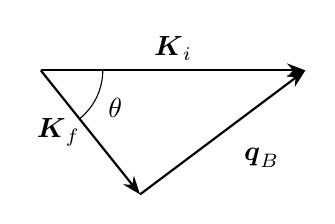
\begin{tikzpicture}[>=Stealth,scale=1.05]
 \coordinate (O) at (0,0); \coordinate (I) at (3.2,0); \coordinate (F) at (1.2,-1.5);
 \draw[->,thick] (O)--(I) node[midway,above] {$\boldsymbol K_i$};
 \draw[->,thick] (O)--(F) node[midway,left] {$\boldsymbol K_f$};
 \draw[->,thick] (F)--(I) node[midway,below right,xshift=4pt,yshift=-2pt] {$\boldsymbol q_B$};
 \draw (0.75,0) arc (0:-51:0.75);
 \node at (0.9,-0.45) {$\theta$};
\end{tikzpicture}
\end{center}
である。$\omega_i\gg\omega_B$ なら $|\boldsymbol K_f|\simeq|\boldsymbol K_i|$ なので
\begin{align}
 |\boldsymbol q_B|^2&=|\boldsymbol K_i|^2+|\boldsymbol K_f|^2
 -2|\boldsymbol K_i||\boldsymbol K_f|\cos\theta\\
 &\simeq2|\boldsymbol K_i|^2(1-\cos\theta),\\
 &\boxed{|\boldsymbol q_B|\simeq2|\boldsymbol K_i|\sin(\theta/2).}
\end{align}

\section*{[5] 音速とBrillouin周波数}
長波長音響フォノンでは $\omega_B=v_a|\boldsymbol q_B|$ である。媒質中の光子波数は $|\boldsymbol K_i|=n\omega_i/c$ だから
\begin{equation}
 \boxed{\frac{\omega_B}{v_a}=\frac{2n\omega_i}{c}\sin(\theta/2).}
\end{equation}

\section*{[6] 音速の数値}
分光波数を $\tilde\nu_B=1/\lambda_B=3.0\,\mathrm{cm^{-1}}=3.0\times10^2\,\mathrm{m^{-1}}$ とする。原本の $\hbar\omega_B=hc\tilde\nu_B$ と $h=2\pi\hbar$ より $\omega_B=2\pi c\tilde\nu_B$ である。また $\omega_i=2\pi c/\lambda_i$ なので $\omega_B/\omega_i=\lambda_i\tilde\nu_B$。散乱角 $180^\circ$ では
\begin{align}
 v_a&=\frac{c}{2n}\frac{\omega_B}{\omega_i}
 =\frac{c\lambda_i\tilde\nu_B}{2n}\\
 &=\frac{(3.0\times10^8)(680\times10^{-9})(3.0\times10^2)}{2(2.4)}\,\mathrm{m/s}\\
 &=1.275\times10^4\,\mathrm{m/s}
 \simeq\boxed{1.3\times10^4\,\mathrm{m/s}}\quad(2\text{桁}).
\end{align}

\section*{[7] 中性子散乱からばね定数}
$q=\pi/a$ では分散関係から
\begin{equation}
 \omega_1=\omega_o(\pi/a)=\sqrt{\frac{2C_1}{m}},\qquad
 \omega_2=\omega_a(\pi/a)=\sqrt{\frac{2C_2}{m}}.
\end{equation}
中性子の運動エネルギー $E_n=\hbar^2K^2/(2M_n)$ と $K=2\pi/\lambda$ を用いる。フォノンを生成するので
\begin{equation}
 \frac{\hbar^2}{2M_n}\left[\left(\frac{2\pi}{\lambda_{ij}}\right)^2
 -\left(\frac{2\pi}{\lambda_f}\right)^2\right]=\hbar\omega_j,
 \qquad j=1,2.
\end{equation}
ここで $\lambda_{i1}<\lambda_{i2}$ なので、同一の $\lambda_f$ に対して $j=1$ のエネルギー移行が大きく、光学枝 $C_1$、$j=2$ は音響枝 $C_2$ に対応する。$\Delta_j=\lambda_{ij}^{-2}-\lambda_f^{-2}>0$ と置けば
\begin{equation}
 \boxed{C_j=\frac{2m\pi^4\hbar^2}{M_n^2}\Delta_j^2,
 \qquad j=1,2.}
\end{equation}

\section*{[8] 格子定数}
音響速度の式を $a$ について解くと
\begin{equation}
 a=v_a\sqrt{2m\left(\frac1{C_1}+\frac1{C_2}\right)}.
\end{equation}
ばね定数の表式を代入して
\begin{equation}
 \boxed{a=\frac{v_aM_n}{\pi^2\hbar}
 \sqrt{\frac1{\Delta_1^2}+\frac1{\Delta_2^2}}},\qquad
 \Delta_j=\frac1{\lambda_{ij}^2}-\frac1{\lambda_f^2}.
\end{equation}
この式は長さの次元を持ち、音速因子 $v_a$ を含む。

\end{document}
